\PassOptionsToPackage{unicode=true}{hyperref} % options for packages loaded elsewhere
\PassOptionsToPackage{hyphens}{url}
%
\documentclass{book}        % from not too short p76 pagestyle
%\usepackage{fancyhdr}
%\pagestyle{fancy}
%ensure chapter section headngs in lower case
%
\usepackage{graphicx}
\DeclareGraphicsExtensions{.png,.jpg}
\usepackage{xeCJK}
\setCJKmainfont{SimSun}
\usepackage{lmodern}
\usepackage{amssymb,amsmath}
\usepackage{ifxetex,ifluatex}
\usepackage{fixltx2e} % provides \textsubscript
\ifnum 0\ifxetex 1\fi\ifluatex 1\fi=0 % if pdftex
  \usepackage[T1]{fontenc}
  \usepackage[utf8]{inputenc}
  \usepackage{textcomp} % provides euro and other symbols
\else % if luatex or xelatex
  \usepackage{unicode-math}
  \defaultfontfeatures{Ligatures=TeX,Scale=MatchLowercase}
\fi
% use upquote if available, for straight quotes in verbatim environments
\IfFileExists{upquote.sty}{\usepackage{upquote}}{}
% use microtype if available
\IfFileExists{microtype.sty}{%
\usepackage[]{microtype}
\UseMicrotypeSet[protrusion]{basicmath} % disable protrusion for tt fonts
}{}
\IfFileExists{parskip.sty}{%
\usepackage{parskip}
}{% else
\setlength{\parindent}{0pt}
\setlength{\parskip}{6pt plus 2pt minus 1pt}
}
\usepackage{hyperref}
\hypersetup{
            pdfborder={0 0 0},
            breaklinks=true}
\urlstyle{same}  % don't use monospace font for urls
\usepackage{longtable,booktabs}
% Fix footnotes in tables (requires footnote package)
\usepackage{multirow} %for tabular combine multirow
\IfFileExists{footnote.sty}{\usepackage{footnote}\makesavenoteenv{longtable}}{}
\setlength{\emergencystretch}{3em}  % prevent overfull lines
\providecommand{\tightlist}{%
  \setlength{\itemsep}{0pt}\setlength{\parskip}{0pt}}
\setcounter{secnumdepth}{0}
% Redefines (sub)paragraphs to behave more like sections
\ifx\paragraph\undefined\else
\let\oldparagraph\paragraph
\renewcommand{\paragraph}[1]{\oldparagraph{#1}\mbox{}}
\fi
\ifx\subparagraph\undefined\else
\let\oldsubparagraph\subparagraph
\renewcommand{\subparagraph}[1]{\oldsubparagraph{#1}\mbox{}}
\fi

% set default figure placement to htbp
\makeatletter
\def\fps@figure{htbp}
\makeatother
\date{}
\begin{document}               % plus the \end{document} command at the end.



``发现我讲过的方法，老是重复再解释，再提醒，是否我教的方法有问题?''
与某老师交流时，对方提出。

``很正常，绝不要怀疑方法本身，我也常常遇到。其实这是所有学习的必经过程：开始时只是初步按学到的技巧用于本项目中，若要能持久，除了需要团队不断实验才能真正理解，离不开：奴、徒、工、匠、师、家、圣
，这不断提升的过程。
但更关键是高层的认同与支持，不然很容易会出现你说的情况。''

\hypertarget{ux9879ux76eeux56e2ux961fux5206ux6790ux6839ux56e0}{%
\subsection{项目团队分析根因}\label{ux9879ux76eeux56e2ux961fux5206ux6790ux6839ux56e0}}

某家专门做企业管理产品的软件开发的Y公司：\\
总经理听我说如能做好迭代回顾、根本原因分析，不但可以能减少大量的后期返工，提升产品质量，也可以提升总体开发效率，很感兴趣。\\
8个月后再碰面，总经理说：``虽然我们现在已经要求团队多做回顾根因分析,
但每次迭代的系统测试缺陷数量还是降不下来，例如某产品线，都大概在50个左右，有试过降到30左右，但后面不久又回到之前的水平。你可否跟我们团队谈谈了解一下？''

\framebox{%
\begin{minipage}[t]{0.97\columnwidth}\raggedright
从他们的数据，缺陷分析，系统测试报告等都能看出，其实他们都没有找到根本原因，只是把缺陷分类，对缺陷的问题症状做了修正措施。

问：第二条根因是什么？\\
答：编码人员把某个参数搞混了；

\begin{description}
\tightlist
\item[]
改进措施：提醒开发人员要注意，避免同类问题再发生
\end{description}

第一条：
测试人员不清楚需求，没有设计出充分的测试用例，导致未能在测试阶段预先暴露问题

\begin{description}
\tightlist
\item[]
改进措施：加强人员的培训，更了解业务需求
\end{description}

问：测试本身是不会产出缺陷的，为什么你们识别测试是根本原因的源头呢？
\strut
\end{minipage}}



以上是团队自以为在复盘时已经分析了根因的例子，但不要误以为经过根因分析培训后便能一帆风顺。

某家专门做医疗软件系统产品的公司，团队都已经经过根因分析培训并一直在迭代回顾时使用。以下是项目团队分享会里的交流：

``第一条根本原因写`开发人员不理解需求，没有按照规格要求，导致后面测试不通过。'请举例说明一下。''

``我们这个项目是系统升级，针对医院医生做手术之前的很多准备工作，不仅仅包括麻醉师，也包括护士、设备等都要准备就绪。而且大小医院要求不同，大医院分工很细，小医院可能同一个岗位负责几个任务。所以要避免这类缺陷，首先要画好所有可能处理的流程图，也要明确有哪些不同的配置项，有那些参数。并需要与熟悉流程的产品经理（甚至医生）确认一下。''

``这些是否都应该归属于需要分析根因的内容吗？还记得我们讲过的KJ分析方法：所有团队成员利用便利贴把所有相关的因素、问题写出来，并在大白纸画上之间的关系，才算做好根本原因分析。你现在写的``根本原因''只是浮在水面上现象。

继续看看对应的纠正措施：记得我们一直强调改进计划必须像做项目一样用WBS分解到不超过五天的任务并把任务分配到负责人，每个任务也必须有明确产出物。如果只写上一个月后由开发组长负责做好，因缺乏实际行动，最终一个月后很难取得效果。''

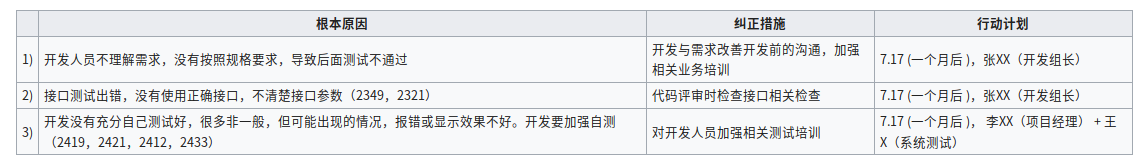
\includegraphics[width=6cm]{Screenshotfrom2024-08-1123-28-39.png}

``我们分析根本原因都应有要数据支撑，不应单依赖个人主观判断。
这里第三项根因只是写了四个缺陷号， 是什么意思？''

``因为我们没有时间把几十条缺陷都列出来分析，我们只能抽几条把缺陷号记下来。''

``你们总共有多少时间做迭代回顾？''

``一小时左右。''

``明白了。确实时间不够，所以管理层必须给你们充分的时间，不然的话，无法做好根本原因分析。''

``第二条写`没有使用正确接口'是什么问题？''

``这系统有很多外部接口与医院现有系统对接，有些缺陷是因为开发一测试用的接口版本不同，导致测试时不通过。''

``记得我们一直强调开发与测试与客户生产环境必须一致，所以这是关于环境的问题，接口只是环境的一部分。为什么会弄错了版本？是否不应单靠人去记录对应哪个最新版本。你们现在代码开发版本在Git管理；但相关文档，包括配置，在SVN管理。依赖人工记录之间的相互对应很容易出错，这才是根因。''

\hypertarget{ux5206ux6790ux5168ux8fc7ux7a0b}{%
\subsubsection{分析全过程}\label{ux5206ux6790ux5168ux8fc7ux7a0b}}

为北京某企业做差距分析，发现大量缺陷在系统测试才被发现，建议加强迭代回顾根因分析。\\
质量经理：你说我们上次做了回顾还没有找到真正根因，但不知道如何改善。\\
我： 数据是根因分析的基础，若要做好分析，首先要有充分和足够数据。\\
例如团队只依据系统测试缺陷数据做分析，因为没有缺陷的返工工作量数据，只能从缺陷类型的数量分析，难以识别出影响最大的缺陷类。

没有考虑从需求设计开始的评审、编码人员自测，也没有考虑各阶段的缺陷排除率，大家便只能从系统测试缺陷的症状分析，结论是编码人员疏忽、能力不足，不会考虑这些缺陷是否可以预先避免和预防；

所以我们每次迭代回顾时，在做分析前必须让团队有足够时间收集数据，画出全流程，识别失效点，对分析也有帮助。

流程图也可以帮助分析过程并找出根因。画了流程图后，便可以利用FMEA方法针对每个失效点找根因和对应纠正措施。

\framebox{%
\begin{minipage}[t]{0.97\columnwidth}\raggedright
某家公司专门为电信供应商做客服管理软件系统，因客户对质量有要求，每次发布后都分析有哪些发版后的问题。有些软件开发相关问题不容易排查根因,例如某次发布后发现报表的数字对不上,但这些错误不是立马使用时就出现，开始的时候没问题但使用时间长了,就会产生错误。\\
团队花了很长时间分析整个过程，最终发现错误是由于有些内部接口，没有考虑到所有传输数据是否正常，有些有错但没拒收,导致开始时没问题,但累积多了就会出现最后的报表错误。最后也针对这问题改正了。\\
讨论分析如何能避免同类问题：

%\href{文件:微信截图_20230928135611.png}{500px}
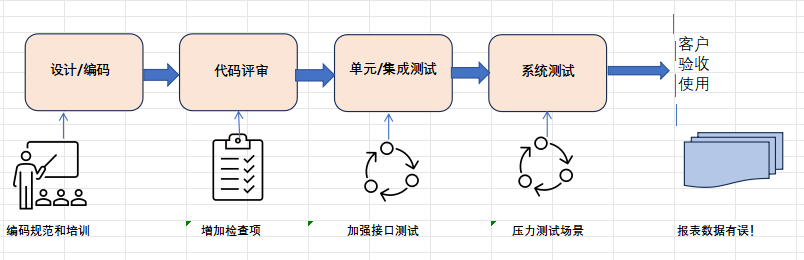
\includegraphics[width=6cm]{微信截图_20230928135611.png}

按系统产品集成的流程,识别有那些点可避免问题发生（FMEA思路）。可以在集成测试时和系统测试时,增加类似的场景，加大类似的压力测试，应可预先暴露问题；集成测试时，如果都测试所有接口传输的数据，也可以避免问题；如果我们前面做好设计和代码的评审（根源与设计有关）,也应该可以避免。例如如果针对这种问题,完善评审检查单的检查项，以后应可避免同类问题再发生。
\strut
\end{minipage}}


从这个实例可以看出，首先绘制总体流程或路线图，并识别每个环节的潜在风险，有助于更好地挖掘问题的根本原因。

除了FMEA方法外，缺陷排除预测模型也可以帮助团队分析从需求到交付的全过程。
如果团队对此不熟悉，可以先安排一天的培训，以帮助他们了解根因分析的重点。

%\href{文件:微信截图_20230830093612.png}{500px}

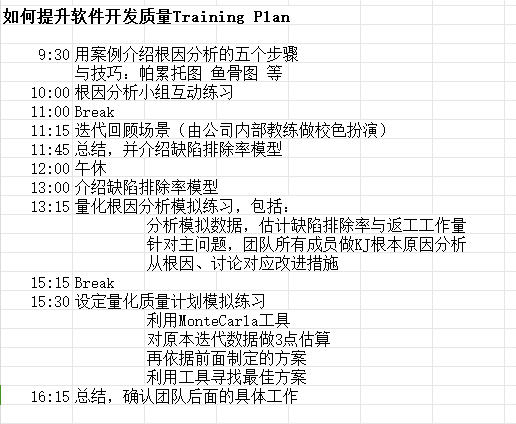
\includegraphics[width=6cm]{微信截图_20230830093612.png}

以上一天培训让团队了解以下重点：\\
\textbf{改进目标}：降低返工工作量（同时也会降低缺陷后期才被发现的数量）\\
\textbf{分析根因}：不仅要分析后期发现缺陷的分类与数量，还需对从需求到最终客户验收的全生命周期进行缺陷排除率分析，以找出最薄弱的环节并深入挖掘根因。利用数据进行互动练习是最有效的学习方式，因此建议从以往的缺陷数据中抽取70-150条进行小组分析。\\
\textbf{预测效果}：以福特8D根因分析框架为例，缺陷排除与返工预测模型可以帮助团队预估新方法的效果（例如，通过代码静态扫描加强代码评审）。
福特8D的8个步骤：\\
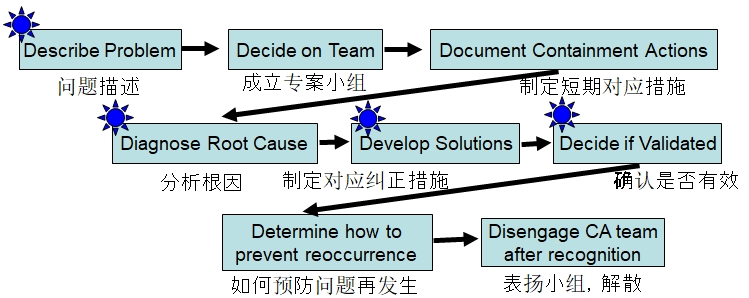
\includegraphics[width=6cm]{CAR_辅导1-1.jpg}

缺陷预测模型可以在分析根因和预估效果步骤里贡献：

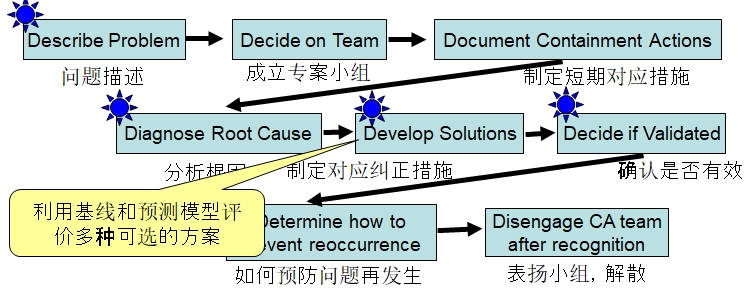
\includegraphics[width=6cm]{CAR_辅导4-1.jpg}

例如，若大部分缺陷集中在系统测试阶段被发现，模型可以预估下一轮迭代中的缺陷分布。如果代码评审发现的缺陷数还没有预期的提升，团队应内部再分析，避免等到系统测试才找出缺陷。（想了解如何利用缺陷排除预测模型预估改进后的效果，详见附件里的“缺陷排除预测模型实例”）

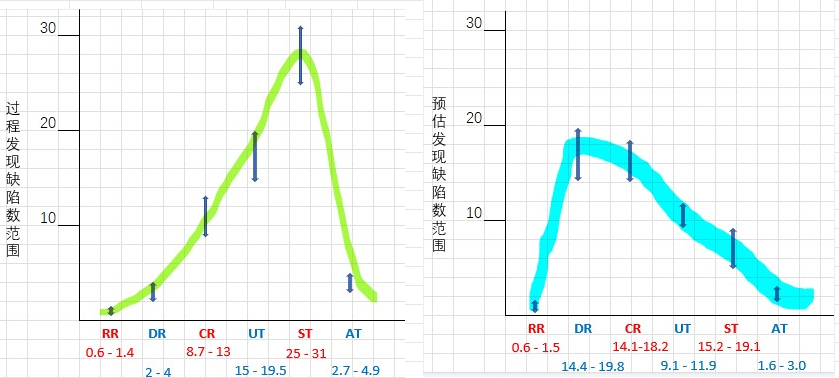
\includegraphics[width=6cm]{MTKL.png}

'''团队自己收集数据'''：此外，团队成员应开始每天或每周自行统计返工的工作量（包括评审缺陷，所有数据均记录在缺陷管理系统中）。

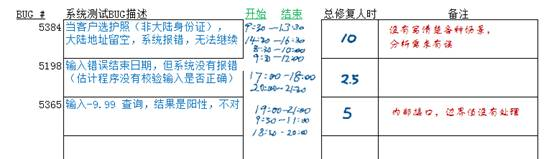
\includegraphics[width=6cm]{缺陷表41.jpg}


\hypertarget{ux5185ux90e8ux6559ux7ec3ux5982ux4f55ux505aux597dux73b0ux573aux8f85ux5bfc}{%
\subsection{内部教练如何做好现场辅导}\label{ux5185ux90e8ux6559ux7ec3ux5982ux4f55ux505aux597dux73b0ux573aux8f85ux5bfc}}

培训后，过了6周，质量经理电话联系我。\\
质量经理：我们计划下周三与项目组进行迭代回顾。该团队有7到8人，两周前曾与另一团队使用便利贴进行了根因分析，确实听到了更多不同的声音。应该如何准备，才能让团队放开并有效地做好根因分析？\\
我：

如果只有缺陷数量和工作量等``硬''数据，但缺乏如团队成员的感受、积极性、主动性等与人性相关的``软''数据，也难以真正分析出能够避免同类问题再次发生的根本原因。
（例如冲刺回顾时用时间表 (Timeline)让大家回想过去4周的经历，并用Color
Code Dots
颜色点让每位成员标上每一事件的感受，是收集软数据方法之一，详见附件：敏捷回顾互动练习）

要做好回顾，准备工作至关重要。例如，需要准备大白纸，并确保有足够的空间。如果团队成员围坐在一个大桌子旁进行讨论，效果往往不佳。相反，如果我们在墙上贴上大白纸，提供便利贴、大号和小号水笔，每个人都有自己的一支笔时，团队成员会更加投入。他们会走动、讨论、写字、画图，并不断交换位置、互相帮助，这样能更好地体现团队精神。

因此，辅导的重点不是在各种技巧上，不是教他们每一步怎么做，只需提醒时间（时间的管理很重要。每次进行小组练习时，我都会用电脑投屏显示剩余时间（分钟），让团队即时掌握剩余的时间）。

先定好目标，让他们团队自己发挥与讨论，效果会更好。只要他们清楚需要做什么，大部分团队都能自行分工，比如有些人负责画帕累托图，有些人做总体根因分析。

质量经理：你的意思是减少干预，尽量让团队自主思考。但因未做过，可否再举些例子？\\
我：正确。不如我反过来，建议你应该避免说什么：

\begin{enumerate}
\tightlist
\item
  其实你们团队和我见到的其他团队相比好或者差（因这都是个人观点、感觉，非事实）。
\item
  本来只需要你们画帕累托图和鱼骨图，为什么你们还画了个脑图？
\item
  你们都已经讨论了很多细节，要立马赶紧时间做最后总结。
\item
  你们讨论好像都只是针对机场闸口的问题，是否应该也考虑其它？
\end{enumerate}

为什么要鼓励团队表达不同意见？

团队要改进，首先要确保成员充分理解彼此的差异。经过充分讨论后，团队成员找到共通点，才有机会一起改进。

如果大家可以在回顾时开放讨论,把自己的具体看法说出来,就可以让大家看到全貌，问题的真正情况。

因此，内部教练应鼓励多样化的声音。心理学家Asch
1951年的从众试验证明，只要有一个人率先提出异议，陆续更多的人也会表达自己的意见。因此，内部顾问应确保每个人都有发声的机会。意见越多样化，大家越能了解真正的问题，找到大家认可的改进方案（详见附件：功能性分组帮助团队成长实例）。

例如，如果发现团队在大型会议上因人数众多而不愿发言，可以考虑分成小组讨论，这通常会更有效。
对于一些``慢热''的团队，需要给予他们更多时间，不要急于打破沉默，等一下。一旦有人开始发言，接下来就好办了。

\hypertarget{ux4eceux8fedux4ee3ux590dux76d8ux5230ux6301ux7eedux6539ux8fdb}{%
\subsection{从迭代复盘到持续改进}\label{ux4eceux8fedux4ee3ux590dux76d8ux5230ux6301ux7eedux6539ux8fdb}}

当某些团队已经能做好回顾根因分析，利用数据改善下一轮开发质量。
如何可以变成团队或公司的持续改进呢？

\framebox{%
\begin{minipage}[t]{0.97\columnwidth}\raggedright

深圳有一家公司专门是做内部IT服务。因为要求很严格，都要经过测试验收都通过，才允许新版本正式投产（发版）。每2周会做一次发版，每次都会统计发版成功率，因为都做了很久，依据以往水平，要求发版成功率不会低于96%，并一直都监控这个百分比趋势。某一个月发现成功率跌到接近96%。质量改进组就开始启动根因分析。先看是哪个部门出问题引起发板率低。发现有两个部门表现最差，然后针对这两部门做根因分析找出具体原因。然后也对应一些原因做了纠正措施，比如培训评审等等，做以后发现确实那些问题解决了。发版率的水平也提升了，后面他反而可以把那个变成新的基线，变成一个新的水平，到了98\%。
 
\strut
\end{minipage}}


个别项目组的迭代回顾能有效改善，只可以是用来让高层关注的``种子''，从工作量和缺陷的改善看到这些持续的浪费确实能大大减少，但如果高层不关注，不投入资源，这类``改善''只是短暂的闪光，很快大家又回到以前的工作状态。

\hypertarget{ux4e0eyux516cux53f8ux603bux7ecfux7406ux6c47ux62a5}{%
\subsection{与Y公司总经理汇报}\label{ux4e0eyux516cux53f8ux603bux7ecfux7406ux6c47ux62a5}}

我与本章第一个案例做企业管理产品的Y公司里的团队交流，了解问题原因后与总经理汇报说：\\
``你不是问我为什么我们的缺陷数量总是降不下来，经过和你们团队沟通，发现了很多都误解了根本原因分析，所以虽然做了复盘，过程和做法和以前都没有有任何变化。''\\
``有什么好建议？''\\
``任何质量改进要有效，必须先从高层的关注和支持开始。
如果管理层认同这改进很重要，对企业有价值就必须当成项目来做，
项目要有高层领导和监督，成立改进小组，指派小组成员，按改进目标定具体任务，并制定项目管理计划，高层每月监督进展。''

``我们高层是非常支持改进的，但我们人员手上的任务都很多，很难要他们腾出时间做计划与监控。既然他们已经有复盘习惯，可否先做些根因分析培训？''

``没有问题，我当然可以按你们安排做培训。开始时某些团队可能会做出些较好的分析，并有效果，但过了几轮，因缺乏公司持续质量改进的支持，不久又会返回原本，因为要改变人的习惯是非常难。''

培训不能改变团队的思路和做事的习惯，虽然培训很重要，但培训本身无法给企业带来可持续质量改善的公司文化。

\hypertarget{ux6539ux8fdbux6548ux679c}{%
\subsection{改进效果}\label{ux6539ux8fdbux6548ux679c}}

某香港A公司成立过程改进小组，并有高层作为组长监督每月小组会议，原先用传统会议形式，
虽然每次都有会议纪要与代办事项， 但过了三个月，没有什么具体进展。
我建议他们再回顾之前培训过的各种根因分析方法，并改用KJ方法大家用便利贴
一起讨论：
开会时每人手拿便利贴，小号笔大家一起围着墙上的大白纸讨论分析并一起制定改进行动和目标。开始时有些反对意见：
``我们之前开会讨论大家都有提出各种意见，不一定要用这方法。''
我解释``当大家都做下来开会讨论，当某人提了意见，其他人如有其他想法，他先要想好如何提，如果对方反对如何对应等，所以一般不太愿意提其他意见。但如果写在纸上就没有这心理顾虑。''

部门经理开始时都是观望，但当他们逐渐看到高层对过程改进有决心，非一时的口号，
也开始关注过程改进小组的工作。 因为项目经理都是过程改进小组的成员，
项目团队迭代回顾也使用便利贴大白纸讨论的方式。

四个月后改进小组组长（高层代表）回顾说
``开始时没有经验，后面改用了便利贴一起互动讨论方式，
看到他们开始愿意积极参与，从每个月完成的改进项数量，
和客户缺陷密度数等都看到逐渐有按月的改进。''

反观世界级企业如丰田汽车，从二战后一直到现在不断持续改善，超越了原本的美国汽车巨头。
``90年代，丰田汽车共8万员工，每年共用4百万条过程改进建议，平均每员工每年有50条。''Dr
Juran
用以上例子什么是企业持续改善文化，也正是这种改善动力让丰田超越竞争对手，成为全球最大汽车公司。

公司持续改善必须有高层的关注并提供资源，把过程改进当成项目来管理。但万事起头难，
有了管理层的支持后，开始时如何能软硬兼施，让他们``动''起来，所谓``解冰''很重要。如果头几个月未能改变他们的习惯，后面便会越来越难。反之，如果能让小组尽快动起来，后面便能逐渐变为像丰田那种持续改善的文化。

\hypertarget{ux9644ux4ef6}{%
\section{附件}\label{ux9644ux4ef6}}

\hypertarget{ux529fux80fdux6027ux5206ux7ec4ux5e2eux52a9ux56e2ux961fux6210ux957fux5b9eux4f8b}{%
\subsection{功能性分组帮助团队成长实例}\label{ux529fux80fdux6027ux5206ux7ec4ux5e2eux52a9ux56e2ux961fux6210ux957fux5b9eux4f8b}}

系统，包括团队、公司的成长都依靠不断集合内部的差异，如果完全不能接受不同意见，就无法进步。基于心理学家
Yvonne Agazarian 系统中心理论 (Systems Centered
Theory)，团队必须先从传统（按岗位、功能）分组(Stereotype Subgroup)
变为功能性分组(Functional Subgroup)，才能成长。\\
要让大家觉得有共同点，基于这基础才可以听从不同意见。

\framebox{%
\begin{minipage}[t]{0.97\columnwidth}\raggedright
 场景实例：\\团队讨论如何完善社区里面的教育，大家讨论个人的希望。\\ 
A：好像我们大家的想法都很类似。\\ 
内部教练：可否举个例子？\\ 
B：我们都想为自己和我们后代有个终身不断学习的机会。\\
C：好像我们都没有人提过大学，不知道为什么。\\
 D：但很多人负担不起大学学费。\\
 E：我觉得每个人只要想受到教育，都能做到，我就是靠自身努力。最后完成大学教育。\\
 F：（开始跟D形成小组）是的，但教育确实越来越昂贵，
我估计我们当中不少人负担不起那些美国东岸名校的昂贵学费。\\ 
G：（有成见，觉得那些不能完成大学教育的都是没有动力，没有上进心）我还是觉得任何人，只要有动力都能做到。\\
 如果没有人附和E的观点，就可能变成他的个人独角戏。后面有两个可能的发展场景：\\
 场景一C 附和了E的观点。\\ 
C：我的经历确实和E说的类似，辛辛苦苦最终完成了大学教育，但确实很艰苦。
如果我当时没有舅舅的支持，肯定完成不了。\\ 
场景二 没有人附和E的说法。\\ 内部教练：有没有其他人也有经过自己努力完成大学教育的经历？\\ （注意：内部教练千万不能说：``有没有人赞同，人只要有动力都能进大学？''因为这只是个人观点，并非事实。）\\
 A：我确实也完成了大学教育了，但也经历了很多困难。\\
 G：我读了一年，因为再得不到奖学金，没有办法，只能退学。\\
到了这个点，整个分组就比较复杂，虽然生成了新小组，
E得到一些回应，但也有些人提出不同的经验，需要有说法把新小组归纳。\\
 接下来，\\
 C：我看来这个很简单，有些人能完成大学教育。有些人虽然很希望完成，最终还是完成不了，但不是所有人都想或者必须完成大学教育。所以我们的改进任务应该是帮助所有人学到他希望学习的东西。\\
 有了以上C的说法，整个团队就可以进一步成长。

\strut
\end{minipage}}

从以上实例看到，首先要让大家愿意接受不同意见，不然的话就会变成争吵，不会有效果。有人提出不同意见后，必须有人附和，成为他的战友，才能形成新的小组。有了新小组以后，团队需要把不同小组的立场合并起来，变成一个新方向、新思路，整个团队就有成长、进步。

\hypertarget{ux654fux6377ux56deux987eux4e92ux52a8ux7ec3ux4e601ux65f6ux95f4ux8868-timeline}{%
\subsection{敏捷回顾互动练习1:时间表
(Timeline)}\label{ux654fux6377ux56deux987eux4e92ux52a8ux7ec3ux4e601ux65f6ux95f4ux8868-timeline}}

在较长的迭代、发布或项目回顾中使用此方法收集数据。

\hypertarget{ux76eeux7684}{%
\subsubsection{目的}\label{ux76eeux7684}}

促进大家记忆，从多个角度回看之前的工作。大家一起回看谁在什么时候做了什么工作，与当初的假设对比。看是否有什么规律？或者生产水平有没有变化？用来表达事实和每人的感受。

\hypertarget{ux6240ux9700ux7684ux65f6ux95f4}{%
\subsubsection{所需的时间}\label{ux6240ux9700ux7684ux65f6ux95f4}}

30到90分钟，这取决于团队的规模和迭代周期长短。

\hypertarget{ux63cfux8ff0}{%
\subsubsection{描述}\label{ux63cfux8ff0}}

小组成员写卡片来标示那些很有印象、特别有意义或其他重要事件，然后按时间顺序贴在时间表
(Timeline)上。教练鼓励团队讨论事件，以了解已发生的事实和感受。

变化：功能性泳道 Functional Swim Lanes \\
沿时间轴的背景线纵向绘制行(假设你不打算直接在墙上张贴卡片，然后使用丝带或胶带划分行)。为每个部门或功能做一行。每组只会把他们的卡片放在自己组的泳道里。

%\url{文件:Timeline.png}

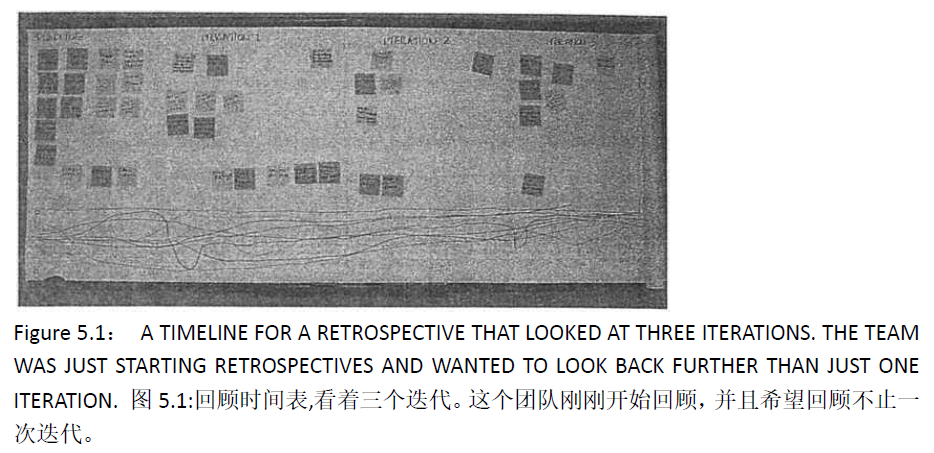
\includegraphics[width=6cm]{Timeline.png}

\hypertarget{ux654fux6377ux56deux987eux4e92ux52a8ux7ec3ux4e602-ux989cux8272ux70b9-color-code-dots}{%
\subsection{敏捷回顾互动练习2: 颜色点 (Color Code
Dots)}\label{ux654fux6377ux56deux987eux4e92ux52a8ux7ec3ux4e602-ux989cux8272ux70b9-color-code-dots}}

与时间表(Timeline)练习结合使用，在更长的迭代回顾中收集团员的感受。

\hypertarget{ux76eeux7684-1}{%
\subsubsection{目的}\label{ux76eeux7684-1}}

展示团队成员对经历事件的感受。

\hypertarget{ux6240ux9700ux7684ux65f6ux95f4-1}{%
\subsubsection{所需的时间}\label{ux6240ux9700ux7684ux65f6ux95f4-1}}

5至20分钟。

\hypertarget{ux63cfux8ff0-1}{%
\subsubsection{描述}\label{ux63cfux8ff0-1}}

团队成员使用颜色点来表示在时间轴上事件的心情高低。
当所有的事件都已经展示在时间轴上，团队也已经回顾后，每人使用颜色点来显示他们的情绪是高还是低(见图)。

\begin{enumerate}
\tightlist
\item
  ``我们已经一起看了事实，让我们也看看大家工作时的心情，状态。''
  作为开始之前说，让大家理解游戏目的。
\item
  给每个人提供两种颜色的点。每人从7到10个点开始，如后面不够用，可提供更多。解释哪种颜色代表情绪高，哪种颜色代表情绪低。
\item
  让每个人都用点来表示哪里情绪高，哪里停滞、衰弱或低潮。
\end{enumerate}

%\url{文件:Color_Code_Dots.png}

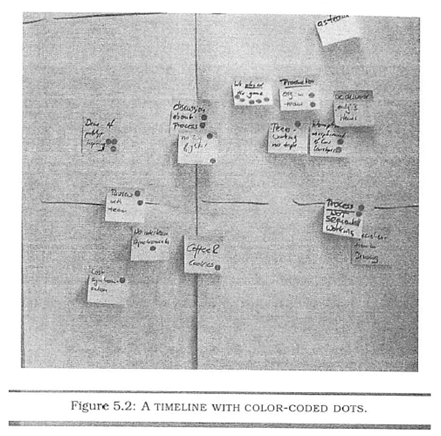
\includegraphics[width=6cm]{Color_Code_Dots.png}

\hypertarget{ux7f3aux9677ux6392ux9664ux9884ux6d4bux6a21ux578bux5b9eux4f8b}{%
\subsection{缺陷排除预测模型实例}\label{ux7f3aux9677ux6392ux9664ux9884ux6d4bux6a21ux578bux5b9eux4f8b}}

\begin{itemize}
\tightlist
\item
  团队分析迭代缺陷数据，缺陷是源自需求/设计/编码，得出以下分布表：
\end{itemize}

%\url{文件:微信截图_20220316093044.jpg}

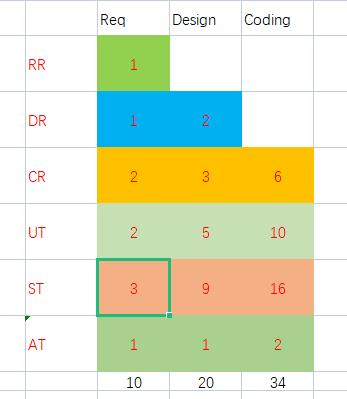
\includegraphics[width=6cm]{微信截图_20220316093044.jpg}

\begin{itemize}
\tightlist
\item
  按缺陷排除率(DRE)公式，计算出各个过程的缺陷排除率，并把参数输进水晶球模型。例如第一行Quality那行：10
  (共有10个缺陷是源自需求）；第二行：10\%
  (需求评审缺陷排除率是10\%）。(本来迭代缺陷参数都标Infosys 识别。)
\end{itemize}

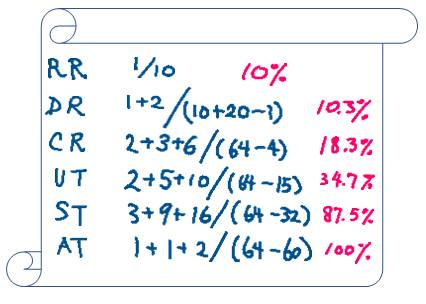
\includegraphics[width=6cm]{2DreEstimateScreenshot_2021-12-01_2120491.jpg}

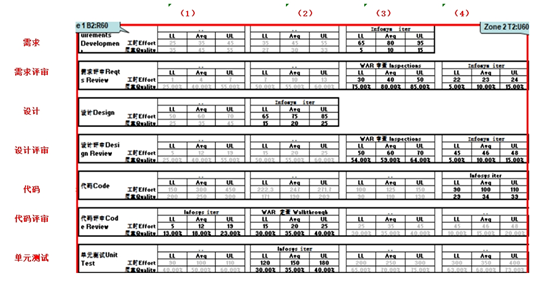
\includegraphics[width=6cm]{Sjb-1-1.png}

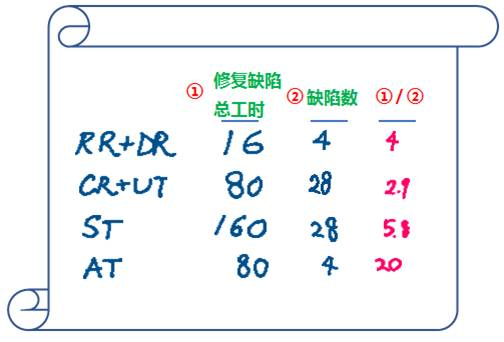
\includegraphics[width=6cm]{4reworkByPhaseScreenshot_2021-12-01_2148381.jpg}

\begin{itemize}
\tightlist
\item
  从团队工时表估算各过程的缺陷返工工作量。例如最下面一行Quality那行输入：\$20,000
  (因为验收测试缺陷平均修复工时是20，假定每工时成本为
  \$1,000）；系统测试那行：\$5,800(因为系统测试缺陷平均修复工时是5.8）。
\end{itemize}

%\href{文件:微信截图_20231031153355.png}{450px}


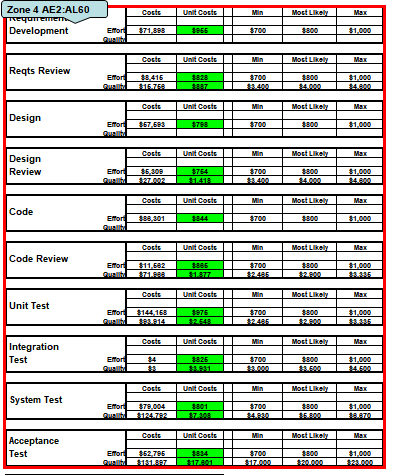
\includegraphics[width=6cm]{微信截图_20231031153355.png}

\begin{itemize}
\tightlist
\item
  估算质量总成本：水晶球会依据质每过程的缺陷分布和单位成本分布，预估质量成本的分布。按本来迭代需求引入缺陷数=10（3），需求评审缺陷排除率等于10\%（4），设计引入缺陷数=20（2），设计评审排除率=10\%（4），代码引入缺陷书=34（4），代码评审排除率=18\%（1），单元测试缺陷排除率=35\%（2），系统测试缺陷排除率=88\%（1），验收测试缺陷排除率=99\%（3）来估算质量成本分布。
\end{itemize}

\begin{itemize}
\tightlist
\item
  如果我们把优化后的缺陷分布与本来迭代的缺陷分布比较（本章正文里比较前后两迭代的缺陷分布左右两图比较），能看出改进后，本来在系统测试才发现的缺陷大多数可以预先在评审暴露，降低返工工作量，也可以预估评审缺陷范围，如果实际评审缺陷数未能达到范围，便可预警，尽快纠正。
\end{itemize}

如果没有预测模型，我们只能主观估计会降低，有了预测模型，便可以估计缺陷分布的变化，也能帮我们挑选最佳搭配，并预估下一轮的缺陷分布范围。

\textbf{解读预测模型最佳搭配选择：}\\
模型以总成本最低可以防止局部最优。例如需求评审没有选用排除率高的新方法，因为新方法会使用较大评审工作量。如果用质量最优（质量成本最低）便必然会读选用缺陷排除率最高的方法，但用总成本来比较便可以综合考虑工作量(Effort)和质量(Quality)，避免局部最优。\\

\hypertarget{ux53c2ux8003-reference}{%
\section{参考 Reference}\label{ux53c2ux8003-reference}}

\begin{enumerate}
\tightlist
\item
  Juran, Joseph. ''Juran's Quality Handbook ''(1999) 5/e\\
\end{enumerate}

\begin{description}
\item[]
\begin{description}
\tightlist
\item[]
-\/-\/-===\textless{}\textless{}\textless{} END
\textgreater{}\textgreater{}\textgreater{}===-\/-\/-
\end{description}
\end{description}

\url{Category:2nd_Ed}

\end{document}
